\section{Daten-Aufbereitung}

\subsection{RADOLAN-Daten}

Die Daten des DWD werden über das Routineverfahren RADOLAN (Radar-Online-Aneichung) erfasst, dass durch eine Kombination von Niederschlagstationen und Wetterradaren hochauflösende Niederschlagsdaten produziert. 

Die Open-Source Bibliothek wradlib \footnote{\url{https://docs.wradlib.org/en/stable/index.html}} stellt für diese RADOLAN-Daten eine Stereographische Projektion zur Verfügung. Dies bedeutet das die Erdkugel zu einem Koordinatensystem aufgespannt wird, dessen Ursprung im Nordpol liegt. Siehe Abbildung  \ref{rz}.

\begin{figure}[H]
	\centering
	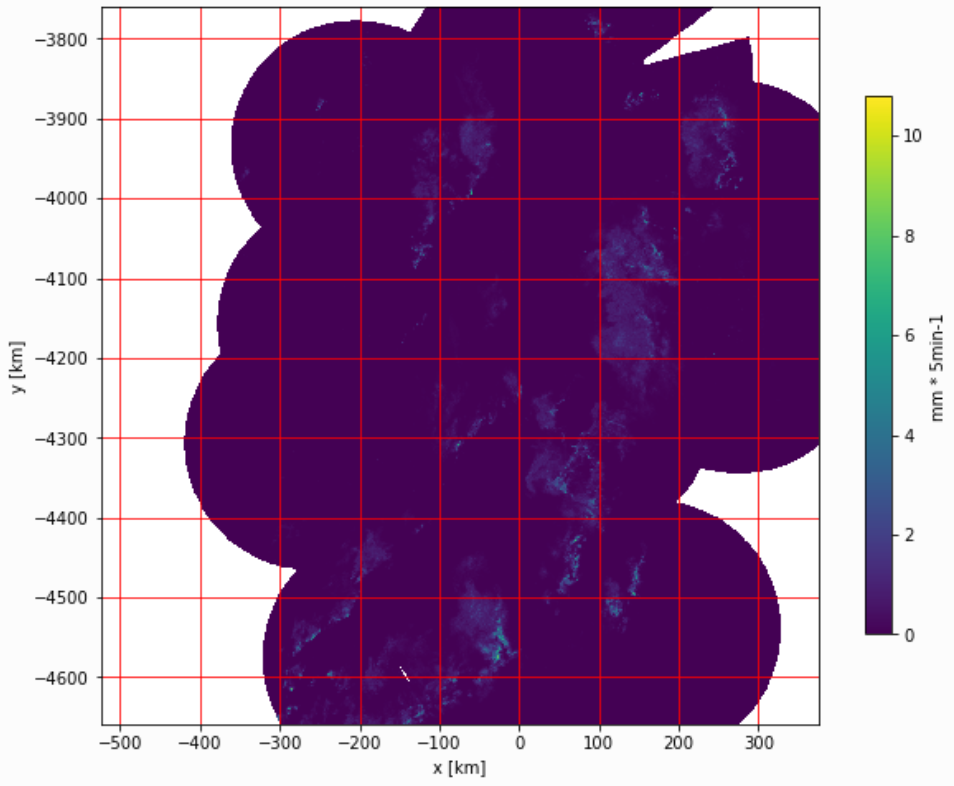
\includegraphics[width=0.8\textwidth]{pics/RZ_product.PNG}
	\caption{Ausschnitt Deutschlands im Koordinatensystem}
	\label{rz}
\end{figure}

Der resultierende Ausschnitt für Deutschland kann mit Hilfe von wradlib als 1100 * 900 Array ausgelesen Werten, dessen Werte einer 1 Kilometer Grid-Box entsprechen.

\subsection{Location Konstanz}
Um für Konstanz und Umgebung sinnvolle Vorhersagen treffen zu können, muss der Standort von Konstanz auf den Daten markiert werden. Dazu müssen die geographischen Koordinaten von Konstanz in X- und Y-Koordinaten des Koordinatensystems umgewandelt werden.

\begin{table}[H]
\centering
\begin{tabularx}{8cm}{X|X}
\multicolumn{2}{c}{Geographische Koordinaten}\\
\textbf{Latitude} & \textbf{Longditude}\\\hline
47.66033          & 9.17582\\
\end{tabularx} 	
\end{table}

\begin{table}[H]
\centering
\begin{tabularx}{8cm}{X|X}
\multicolumn{2}{c}{XY - Koordinaten}\\
\textbf{X-Koordinate} & \textbf{Y-Koordinate}\\\hline
-4602.6447            & -66.4622\\
\end{tabularx} 	
\end{table}

Die umgewandelten XY-Koordinaten müssen nun innerhalb des Arrays gefunden werden. Dazu wurde über den Array iteriert und die Werte mit den errechneten Werten verglichen. Anschließend muss die Location auf der Karte markiert und dargestellt werden (siehe Abbildung~\ref{fig:location}).

\begin{figure}[H]
	\centering
	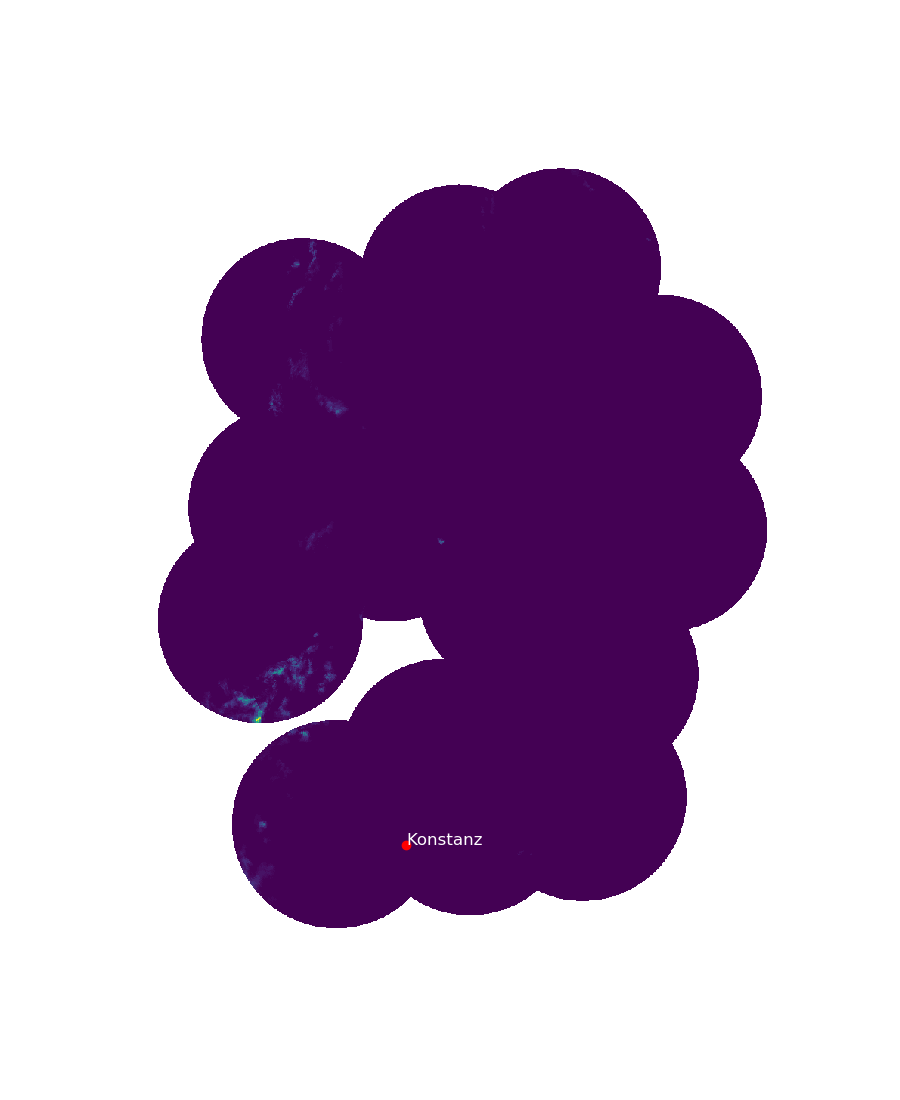
\includegraphics[width=0.8\textwidth]{pics/Location.png}
	\caption{Location von Konstanz im Ausschnitt Deutschland}
	\label{fig:location}
\end{figure}

\subsection{Herausforderungen} 
Änderungen der Auflösung des Formats anpassen, richtige Datenquelle in wradlib finden. XY-Koordinaten innerhalb des Arrays finden und darstellen.
